\DocumentMetadata{testphase=new-or-1}
\documentclass[letterpaper,8pt]{extarticle}  % "extarticle" gives more global font size options. use 8pt with Montserrat and 10pt with EBGaramond
\usepackage{import}
\usepackage{local}
\usepackage[left=.95in,top=.65in,bottom=.75in,right=.85in]{geometry}
\usepackage{lipsum} % to generate text

\title{Can inverse calibration help improving process-explicit species distribution models?}

\author{%
\textbf{Victor Van der Meersch\textcolor{Accent}{\textsuperscript{1*}}, %
Isabelle Chuine\textcolor{Accent}{\textsuperscript{1}} %
}\\
\begin{small}\textcolor{Accent}{\textsuperscript{1}}CEFE, CNRS, Univ. Montpellier - 34000 Montpellier, France \\ 
\textcolor{Accent}{\textsuperscript{*}}Correspondence: \textcolor{Accent}{victor.vandermeersch@cefe.cnrs.fr} \\ \end{small}
}


\date{}
\begin{document}

\maketitle

\section*{Abstract}

\begin{doublespacing}
\begin{linenumbers}

\noindent
\textbf{
Process-explicit models (PEMs) are expected to provide more reliable projections of species range shifts because they explicitly model biological mechanisms that govern species response to climate.
However, this kind of approach requires detailed and diverse data, which are available only for few species. 
Inverse calibration has been identified as an avenue to help calibrating PEMs for many species---yet it is still unclear whether it can yield correctly specified parameters.
Here, we explored the potential of such inverse calibration techniques to enhance the accuracy of PEMs. We calibrated a species distribution PEM which makes a strong focus on phenology and stress resistance using species distribution data, following two strategies: (i) calibrating all parameters simultaneously or (ii) focusing only on critical parameters. We then evaluated the realism of the parameter estimates obtained by comparing them to measurements and comparing simulated phenology to observed phenology across Europe. 
We showed that model structure alone do not sufficiently constrain the calibration process, which may produce unrealistic parameter values. However, using inverse calibration parsimoniously can improve model performance while still allowing to simulate realistic processes.
}

%\begin{multicols*}{2} % if you want two columns
%%%%%%%%%%%%%%%%%%%%%%%%%%%%%%%%%%%%%%%%%%%%%%%%%%%%%%%%%%%%
\section{Introduction}

% Isabelle: give a more general point of view? 
% How to better calibrate models, incorporate more data, to make the most of all the data and knowledge available? And quantify the relevant ecological drivers... to assess species vulnerability

% Marta Benito: trait-based SDMs, refine SDM with measurements from large networks of common gardens - https://doi.org/10.1111/nph.15716, + more transferable https://nsojournals.onlinelibrary.wiley.com/doi/full/10.1111/ecog.05179 ?
% Using mechanistic model outputs as predictors, e.g. https://doi-org.inee.bib.cnrs.fr/10.1111/gcb.13454...
% Compare statistical model ability to reproduce the output of a PB model ("perfect model approach") of crop yield -> statistical models are usefull, in particular are at broader spatial scales (https://doi-org.inee.bib.cnrs.fr/10.1016/j.agrformet.2010.07.008)
% blend mechanstic and phenomenological approaches: https://link.springer.com/article/10.1007/s10980-013-9927-4, to keep mechanistic models tractable, OR https://onlinelibrary.wiley.com/doi/full/10.1111/gcb.13570

% Isabelle: there are many different models, maybe we should focus on parameter estimation -  the problem has more to do with parameter values than process representation? (but recent improvement in plant hydraulics modelling, still a lack of knowledge about dormancy... ?)
% I don't know if I really agree: see https://doi-org.inee.bib.cnrs.fr/10.1038/nclimate1916 
% => a greater proportion of the uncertainty is due to variations among crop models, even after calibration with  same grain yield and growth dynamic data 
% => AND Lack of clarity about hypotheses + re-examination of basic processes, reduction of complexity and increased transparency are all necessary for progress (Harrison et al 2021...)

% "Model parameter estimation tends to be ad hoc and is frequently based on single values"
% "the incorporation of new processes often increases further the number of poorly known parameters that need to be specified"

There have been repeated calls for focusing efforts on the development of process-explicit models (PEMs) in ecology \citep{Urban2016, Singer2016, Pilowsky2022}. Because they describe cause-to-effect relationships, they may provide more robust projections in novel climatic conditions \citep{VanderMeersch2024}. However, PEMs are still applicable to few species \citep{Evans2016}, and their widespread use would first require to address and to quantify their error and uncertainty.

We can distinguish two main source of errors in ecological models: the model's structure and the value of the parameters. The structure of a model is defined by its underlying assumptions and level of simplification. Our understanding of the regulation of the ecophysiological processes at the scale of organisms---that ultimately drive  ecosystem dynamics---has grown substantially in the last decades. This has led to significant improvements in how we represent these processes in models, e.g. plant hydraulics \citep{Ruffault2022} , although some remains challenging, e.g. bud dormancy \citep{Chuine2016} or carbon allocation. 
These advancements enable researchers to explore complex interacting mechanisms, providing useful insights and tools for determining conservation and management strategies in a changing world \citep{Urban2016}. However, the incorporation of new detailed processes can become a trap \citep{Franklin2020}, as it often increases the number of poorly known parameters and limits the number of species for which these models can be applied to. %parameter burden!

Process-explicit modeling depends a great deal on the calibration and the availability of data \citep{Cabral2017}. In a classical framework, parameters are typically determined from experiments, measurements, and expert knowledge. When it is too difficult or impossible, a cost-effective solution to the problem of estimating many parameters is the use of inverse modeling to bridge observations and simulations \citep{Evans2016}. This involves adjusting the parameters until the model outputs closely match the observed data, often using an optimization algorithm. Resulting parameter values are therefore conditional on the structure of the model  and the observed data: the model structure explicitly constrains how climatic factors determine species performance, and the parameters and simulation outputs depend on the observations in a similar way to statistical models \citep{Zhang2024}. Inverse modeling is increasingly used in PEMs to infer model parameters or at least some of them. Process-related data can be used to fit some part of the models separately or sequentially, e.g. tree ring series have been used to calibrate a sapwood growth submodel \citep{DeCaceres2023}, and phenological records are frequently used to calibrate phenological submodels \citep{Chuine2013}. Several data sources can also be combined to refine models \citep{BenitoGarzon2019} and to calibrate several processes simultaneously in a model-data fusion fashion \citep[e.g.][]{Trotsiuk2020}. This allows to integrate data at multiple spatiotemporal scales \citep{Hartig2012, Niu2014}, and reduce potential overfitting issues \citep{Bacour2023}.

However, being able to reproduce observed data, even from several sources, does not guarantee convergence towards biologically sound parameter estimates. First, models are a simplification of reality for several reasons. They often target particular processes that are important for addressing specific questions within a specific spatiotemporal context, and some processes may be unknown or not completely understood. Whether intentional or not, this simplification may miss important processes \citep{Forrester2021}, and inverse calibration may thus lead to parameter values that compensate for these missing processes. Second, even in a structurally correct model, measurements are not likely to coincide precisely with what the model simulates \citep{Zhang2024}. Third, some parameters might also be model-specific (i.e. conceptual), and not correspond to something observable nor measurable.

Process-explicit species distribution models have rarely used inverse modeling with species distribution data available across large scales \citep{Higgins2012, VanderMeersch2023}, probably because this does not align well with the general idea of this modeling approach. Traditionally, these data have only been used by correlative niche models. Yet, the large and constantly increasing volume of such data \citep{Feng2022} represents a vast amount of information that could help improve the accuracy of PEMs \citep{Evans2016}. While using only species occurrence data to infer the values of many parameters can be seen as a brute-force approach, such inverse calibrated PEMs may outperform correlative models and better reproduce the distributional patterns of the species on different spatio-temporal situations \citep{Higgins2020, VanderMeersch2024}.  Moreover, such inverse calibration could also help making PEMs easier to apply to a greater number of species and on a larger scale \citep[e.g.][]{Conradi2024}. However, a good model fit to observations, even long-term data series, does not necessarily imply a good estimation of the processes truly responsible for the observations. 
% To reach high levels of confidence in model projections,  \cite{VanderMeersch2024} showed that ecological processes should still be simulated with a high level of mechanistic realism and that using species occurrence data alone to calibrate models may not provide the highest model performance, especially in novel conditions. 

Here, we investigate the differences between parameter estimates of a PEM obtained either with a classical calibration or with inverse calibration, and what it implies in terms of realism of the simulated processes and of model performance. More precisely, we seek to understand whether and to what extent inverse calibration using species occurrence (i) can lead to realistic parameter values and processes and (ii) may help us improving PEMs. To do this, we focus on PHENOFIT, a PEM which has been used to study species range determinants and to forecast species distribution shifts with past and future climate change in North America and Europe
\citep{Morin2007, Saltre2013, Saltre2015, Cheaib2012}. We first examine in detail 100 calibrations obtained for European beech (\emph{Fagus sylvatica} L.), and analyze the compensations between parameters and the realism of the simulated processes against observations all over Europe. We then investigate whether inverse calibration could improve parameter value estimation of some processes for which data are lacking for eight European forest tree species. 


%\cite{Higgins2012} modified a simple theoretical model of plant growth (initially without environmental forcing) with flexible (mostly empirical?) functions to take into account monthly bioclimatic variables. The parameters of this model were then inferred using a differential evolution genetic algorithm. It has been shown to perform better than a common correlative species distribution model outside the spatial domain used for model calibration \citep{Higgins2020}. 
% The model was designed specifically for this inverse modelling experiment: it uses only monthly environmental variables, and thus has a relatively low complexity compared to the majority of other process-explicit approaches. 
%In the same spirit, \cite{VanderMeersch2023} calibrated PHENOFIT, a more complex model running at a daily step, using only species distribution data. Model was treated as a black box, and a powerfull evolutionnary algorithm (CMA-ES) was used to optimize parameter values. This "fitted" PHENOFIT achieved a high goodness-of-fit (AUC~0.9) during calibration, and was then shown to outperform several correlative models in predicting past vegetation dynamics over the Holocene, in very dissimilar climatic conditions \citep{paperrobustnesspubliéunjourinchallah}. 



%In particular, PHENOFIT was not specifically designed for inverse calibration. The classical way of using the model is to run simulations with an "expert" set of parameter values (determined mainly from experiments and measurements), and most processes simulated within the model can be confronted with field data. 
%It thus offers a great opportunity to investigate the differences between these parameters (\emph{best-guess} estimates) and those inferred using inverse calibration, and what it implies in terms of simulated processes and model performances. Here, we examine in detail these discrepancies to understand whether and to what extent inverse calibration using species occurrence (i) can lead to realistic parameters and processes and (ii) may help us improving process-explicit models. To do this, we first examined in detail the calibrations obtained for \emph{Fagus sylvatica} in \citet{VanderMeersch2023}, analyzing the compensations between parameters and the realism of the simulated processes against observations all over Europe. We then investigated whether inverse calibration could facilitate parameter value estimation of some processes for which we lack data, by using CMA-ES to improve eight species parameter sets. ...

% Few initial ideas:
% => compensate for missing information + compensation between processes\\
% => missing process OR problems with some submodels?\\
% => bias in the data?\\
% => what can we learn from such large scale data?
% => crossing scales?  inform and better constrain critical niche parameters?
% => is the process model used appropriate?

%$\rightarrow$ are the parameter values realistic? \\
%$\rightarrow$ to what extent can we use inverse calibration to improve models? \\


%(\Cref{fig:1A,fig:1B})


%-------------------------------------------------------------------%
\section{Materials and Methods}

\subsection{Process-explicit modeling with PHENOFIT}

PHENOFIT is a process-explicit model developed for temperate tree species which has been used to project their distributions using climatic conditions. It estimates the probability of presence of an adult tree (i.e. fitness), defined as the product of the probability to survive frost and drought events (survival), the proportion of flowers/fruits not killed by frost events (fruit index), and the probability that fruits reach full ripening (maturation index) at a yearly time step (Figure S1).

Each phenological event (leaf unfolding, flowering, fruit maturation and leaf senescence) is simulated with daily climate forcing, and the model assumes that a tree species range depends mainly on the synchronization of its timing of development to the local abiotic conditions and especially the occurrence of some abiotic stresses. Thus, for example, the fitness can be reduced when a severe drought event occurs between budburst and leaf senescence, or when a substantial proportions of leaves and flowers that take part to the development of the fruits are killed by frost. In the following, we will provide a more detailed description of three important processes of PHENOFIT, which will be discussed further in this article. A precise description of the submodels and the response functions can also be found in Supplementary Material for beech.

\subsubsection{Leaf unfolding and flowering submodels}

Dates of leaf unfolding (date at which 50\% of leaves are unfold) and flowering (date at which 50\% of flowers are mature) are calculated using mechanistic phenology models \citep{Chuine2017}. Organ development is represented by a state variable, $S$ for development state, which is the integration of development rates ($R$) over time (in daily steps) from a start date $t_0$. The general structure of mechanistic phenology models for one specific development phase is the following:
$t_n$ such that $S_{n,t}$ = $\sum_{t=t_{n-1}}^{t_n} R_{n,t}$ = $S_n^*$ 
where $n$ is a development phase, $S_{n,t}$ is the state of development on day $t$ in phase $n$; $t_n$ is the end of phase $n$ and  $t_{n-1}$ the end of phase ${n-1}$, $R_{n,t}$ is the rate of development during phase $n$ on day $t$ which is a function of  temperature, and $S_n^*$ is the critical state required to reach $t_n$.  Several phases of development can be modeled in a single model composed of several submodels, each one describing a specific phase such as dormancy induction, endodormancy, ecodormancy, etc. In such case, phases either follow each other sequentially or can overlap depending on the development phase and the species. Leaf unfolding and flowering dates have been modelled here using 2-phases models describing both the bud endodormancy phase (bud remain dormant despite meteorological conditions that could sustain cell growth) and the ecodormancy phase (bud cell growth depends on the meteorological conditions).  Development rates ($R$) are response functions to daily temperature that can be linear or nonlinear (usually with a single optimum), and vary with the species and the development phase. 

% This model, called UniChill, is a sequential two-phase model (endodormancy and ecodormancy phases).  The endodormancy phase begins at day $t_0$. The daily rate of chilling $R_c$ is defined as a threshold function of the daily mean temperature $T_d$:
% \begin{linenomath*}
%     \begin{equation}
%         R_c(T_d) = \left\{ \begin{array}{ll}
%       0 & T_d \geq T_b \\
%       1 & T_d < T_b \\
%     \end{array} 
%     \right.
%     \end{equation}
% \end{linenomath*}
% where $T_b$ is the threshold temperature below which the bud  accumulates chilling units. The endodormancy releases when the accumulated rate of chilling has reached the level $C_{crit}$.

% Then, the ecodormancy phase begins. The daily rate of forcing $R_f$ is defined as a sigmoid function of the daily mean temperature $T_d$:
% \begin{linenomath*}
%     \begin{equation}
%        R_f(T_d) = \frac{1}{1 + e^{-d_T(T_d-T_{50})}}
%     \end{equation}
% \end{linenomath*}
% where $d_T$ is the slope and $T_{50}$ the mid-response temperature. Bud break occurs when the accumulated rate of forcing has reached the level $F_{crit}$.

% Thus, the UniChill model has 6 parameters: $t_0$, $T_b$ and $C_{crit}$ for the first phase, $d_T$, $T_{50}$ and $F_{crit}$ for the second phase. 

\subsubsection{Frost hardiness submodel}

Frost hardiness of vegetative and reproductive organs is modelled according to \citet{Leinonen1996}, as a function of the additive effect of photoperiod and temperature, and depends on the state of development (or phenological state): hardiness varies dynamically between a maximum value reached during bud winter dormancy and a minimum value reached at bud break and flowering. The model has several parameters, including the minimum level of frost hardiness ($FH_{min}$) and the maximum increase of frost hardiness ($\Delta FH_{max}$) conveyed both by photoperiod and temperature. The maximum potential level of frost hardiness is thus $FH_{min}+\Delta FH_{max}$ (see Supplementary Material for a detailed description of the model). 

\subsubsection{Fruit maturation submodel}

Fruits development is modeled with a two-phases mechanistic phenology model:  a first phase of cell multiplication and growth, and a second phase of photosynthetic assimilate accumulation. This second phase is the most important, and depends on several components including the proportion of leaves that resisted frost, water availability and photosynthetic activity. The latter varies according to temperature conditions following the unimodal function of \citet{Wang1998} which involves an optimal temperature parameter $T_{opt}$.  Fruit maturation is integrated over time at the scale of the tree crown, following a normal distribution. The mean date of fruit maturation corresponds to the date when fruit development reaches $Mat_{moy}$, and correspond to the stage 50\% of fruits are ripe,  and fruit maturation starts at $Mat_{moy}$ $-3\sigma$ and ends at $Mat_{moy}$ $+3\sigma$.

\subsubsection{Leaf senescence submodel}
Leaf senescence date (date at which 50\% of leaves have changed color or have fallen) is modelled using a 1-phase mechanistic phenology model with different response functions to temperature and to day length depending on the species \citep{Delpierre2009}. 

\subsection{Model calibration}

\subsubsection{Expert calibration}

PHENOFIT has been calibrated for several European tree species, and validated  by comparing their historical and Holocene distribution to the simulated fitness used as a proxy of species probability of presence  \citep{Saltre2013, Duputie2015, Gauzere2020, VanderMeersch2024}. Some parameters were directly measured or found in the literature, e.g. the frost hardiness submodel parameters. Phenology submodel parameters were inferred by inverse modelling using phenological data across Europe (provided through the TEMPO data portal \url{data.pheno.fr}, and the PEP725 database \url{pep725.eu}). %Finally, a few parameters are prescribed based on expert knowledge as no data to estimate them exist. 
This expert calibration of the model does not involve species occurrence data at any point.

\subsubsection{Inverse calibration with CMA-ES algorithm and species occurrence data}

Following \citet{VanderMeersch2023}, we calibrated PHENOFIT using the covariance matrix adaptation evolution strategy (CMA-ES), which  is a robust algorithm for complex optimization problems \citep{Hansen2001}. It is inspired by Darwin's theory of evolution to find the most fit parameter sets. We ran the CMA-ES calibration on the multicore cluster GenOuest (\url{genouest.org}).

The objective function for the calibration was the area under the receiver operating characteristic curve (AUC), to maximize model discriminating capacity (i.e. potential to distinguish between species presences and absences). To compute the AUC, we used the same occurrence data as in \citet{VanderMeersch2023}. These were mainly extracted from the EU-Forest dataset \citep{Mauri2017}, completed with presence records extracted from the Global Biodiversity Information Facility (\url{gbif.org}) to account for tree occurrences outside forests. We removed GBIF occurrences outside natural species ranges as defined by Atlas Flora Europeae \citep{AFE2005} and EuroVegMap \citep{EVM2003}. The EU-Forest cells where the species is not reported present were considered as (pseudo-)absences. In order to reduce calibration computational costs, we selected subsets of 1000 presences and 1000 absences. Presences were sampled based on a k-means clustering to make sure that all species environmental preferences were proportionally represented (see \citet{VanderMeersch2023} for details). 

First, we ran one hundred calibrations for \emph{Fagus sylvatica}, using species occurrences and the same parameter bounds as in \citet{VanderMeersch2023} in order to remain in realistic parameter ranges. These calibrations are called \emph{full} inverse calibrations in the following (all parameters optimized at once, Figure S2). Second, we ran a second set of inverse calibrations, for eight different species (\emph{Abies alba}, \emph{Betula pendula}, \emph{Fagus sylvatica}, \emph{Fraxinus excelsior}, \emph{Larix decidua}, \emph{Picea abies}, \emph{Quercus pubescens} and \emph{Quercus robur}), to optimize only a subset of parameters. These parameters corresponded to processes that we identified as responsible for false absence errors in the predictions of the expert calibration version of the model---i.e. cases where simulated fitness was low despite the species being present. To identify these processes, we calculated the relative contribution of the three sub-components of fitness: survival ($S$), fruit index ($Fr$) and maturation index ($M$) to the simulated fitness ($F$). The relative contribution of a factor was calculated as the ratio of the product of the two other factors over the total sum of all possible two-factor products. For example, the contribution of survival $S$ was calculated as: $\frac{Fr*M}{S*Fr+S*M+Fr*M}$. Other parameters---corresponding to processes that we did not identified as responsible for false absence errors---were fixed at the expert values. For each species, we ran 5 calibrations on 2 different occurrence subsets (i.e. 10 repetitions). These calibrations are called \emph{partial} inverse calibrations in the following. 

\subsubsection{Climate and soil data used to calibrate and run the model}

Simulations and calibrations were run with climate variables extracted from the ERA5-Land hourly dataset \citep{MunozSabater2021}, for the period 1970-2000. As in \citet{VanderMeersch2023}, we computed daily mean values of several variables: temperatures (minimum, mean and maximum), dewpoint temperature, precipitation, global radiation and wind speed. Daily potential evapotranspiration was calculated using the standard FAO Penman–Monteith equation \citep{Allen1998}. Soil water holding capacity was calculated with the field capacity and wilting point data from EU-SoilHydroGrids \citep{Toth2017} and the percentage of coarse fragments from SoilGrids250m \citep{Hengl2017}.

To assess the similarity between the different calibrations in climatic conditions that differ significantly from those used for calibration, we also ran paleosimulations, using the same climatic forcing as in \citet{VanderMeersch2024}. For this, daily data were generated with the GWGEN wheather generator \citep{Sommer2017}, from the monthly simulations of HadCM3B-M2.1 coupled general circulation model \citep{Armstrong2019}.

\subsection{Parameter estimates' evaluation}

We partitioned the 100 \emph{full} inverse calibrations of \emph{Fagus sylvatica} using two k-means clustering procedures in a row (\Cref{fig:2}). The first clustering was based on the simulated leaf dormancy break and leafout dates. Then, within each cluster, the second clustering was computed based on the fruit maturation and leaf senescence dates.

In order to verify that the parameter values after calibration lead to realistic processes, we calculated root-mean-square errors between simulated phenological dates and observed dates. The latter were extracted from two databases, PEP725 and TEMPO, covering the period 1970-2000, essentially in Central Europe (Figure S3). For \emph{Fagus sylvatica}, we used 59484 observations of leafout, 10449 of flowering, 23606 of fruit maturation and 71469 of leaf senescence (\Cref{fig:3}). Moreover, we used 16329 obs. of \emph{Betula pendula} flowering, 21813 obs. of \emph{Picea abies} flowering and N. obs of \emph{Quercus robur} fruit maturation (\Cref{fig:5}).

% Clustering des calibrations...\\
% Main limiting factors (fig4)...\\

\begin{figure}[h]
\centering
\begin{subcaptiongroup}
\phantomcaption\label{fig:1A} 
\phantomcaption\label{fig:1B}
\phantomcaption\label{fig:1C}
\phantomcaption\label{fig:1D}
\phantomcaption\label{fig:1E}
\end{subcaptiongroup}
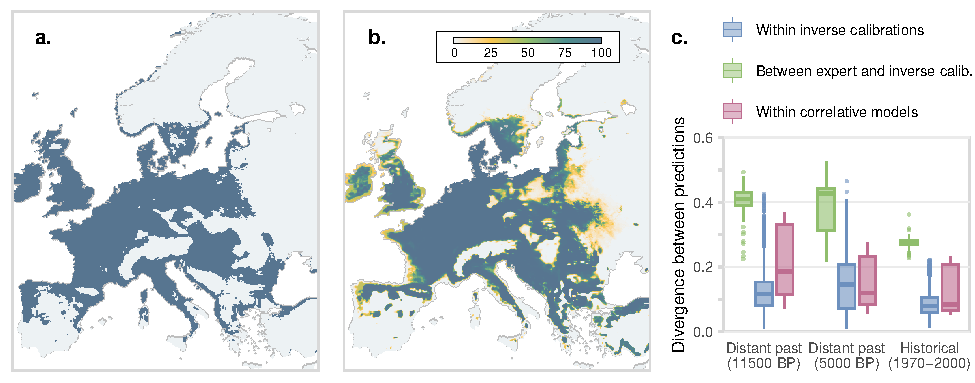
\includegraphics{fig1-1.pdf}
\caption{Simulated potential presence of \emph{F. sylvatica} with \textbf{(a,c)} the expert parametrization and \textbf{(b,d)} the set of 100 \emph{full} inverse calibrations, in the historical climatic conditions \textbf{(a,b)} and in the paleoclimatic conditions \textbf{(c,d)}. Simulated fitness is converted to presence/absence (blue/grey) using the optimal threshold that maximizes the true skill statistic (TSS). \textbf{(e)} S\o rensen dissimilarity between inverse calibrations, and between expert calibration and inverse calibrations. S\o rensen dissimilarity between 5 different correlative species distribution models (from \citealp{VanderMeersch2024}) is shown for comparison. BP stand for "Before Present" (i.e. 1950).}
\label{fig:1}
\end{figure}



\section{Results}

\subsection{Coherent and stable predictions despite process discrepancies}

The similarity between the simulated ranges of European beech obtained with the 100 \emph{full} inverse calibrations was relatively stable over the last 12k years. The disagreements were mostly at the margins of the distribution (\Cref{fig:1B,,fig:1D}). The S\o rensen dissimilarity between the inverse calibration projections was lower in historical conditions (median = 0.0805 [IQR = 0.0605 - 0.106]) than in the distant past, e.g. 11500 years ago (0.116 [0.0813 - 0.154], \Cref{fig:1E}). However it increased relatively little while moving back to the past, i.e. to more dissimilar climatic conditions, compared to the dissimilarity between expert calibration and inverse calibrations, from 0.276 [0.268 - 0.283] in the present to 0.410 [0.391 - 0.429] at 11500 BP.

The relatively similar projections of the 100 \emph{full} inverse calibrations, however, resulted from simulated biological processes that differed substantially (\Cref{fig:2}). Regarding bud development, 65 calibrations (clusters blue and green, \Cref{fig:2A})  had a short endodormancy phase (ending in November or December of the previous year, \Cref{fig:2B}) and a longer ecodormancy phase (with an average duration of 187 days $\pm$ 56.9). On the contrary, the remainder of the 34 calibrations (clusters yellow and orange, \Cref{fig:2A}) had a longer endodormancy phase (ending in February or March) and a shorter ecodormancy phase (with an average duration of 89.4 days $\pm$ 38.7). Note that one of the calibrations stood out due to both short endodormancy and short ecodormancy (\Cref{fig:2B,,fig:2C}). Similarly, two behaviors can be identified in terms of fruit maturation: 83 calibrations (clusters green and yellow) led to early maturation (August/September, \Cref{fig:2D}), and 16 led to late maturation (October/November, \Cref{fig:2D}).

%\begin{itemize}

% \item Agreement between calibrations, relatively stable in different conditions than calibration (maps + similarity index), \emph{F. sylvatica}\\
% $\rightarrow$ divergences from default/classical/expert

% \item But quite different parameter values obtained, and resulting processes\\
% do we get a narrower range than the prior range ?\\
% $\rightarrow$ Figure: selected parameter distribution, associated boxplots on dates with clusters


\subsection{Errors in the simulated processes}

These strong discrepancies between simulated processes inevitably led to differences in terms of agreement with phenological observations across Europe (\Cref{fig:3}). The first group of calibrations (short endodormancy/long ecodormancy) had a median error of 28.3 days for the budburst date, and up to 120 days for the worst calibration. The second group (long endodormancy/short ecodormancy) had a smaller median error of 16.3 days [7.73 - 27.4]. Both performed worse than the expert version of the model (6.95 days [3.36 - 12.1], \Cref{fig:3A}) whose parameters were calibrated using some of these observations. Regarding fruit maturation, the late-maturation cluster (blue and orange) got a median error of 17 days [8 - 29], closer to the expert version (13 days [6 - 24]). Moreover, inverse calibrations showed almost no year where fruit maturation could not occur unlike the expert version, whose parameters did not allow for ripe fruits in more than 50\% of the cases (\Cref{fig:3C}). For leaf senescence, contrary to the expert version which always predicted a senescence date, 43\% of the calibrations led to no senescence date for at least 50\% of the cases (\Cref{fig:3D}), and 34\% to no senescence at all. These calibrations belonged exclusively to the early-maturation cluster (green and yellow), whereas the late-maturation cluster got a median error of senescence date of 14.6 days [8.75 - 22], slightly higher than the expert version (10.8 days [6 - 16]).

\begin{figure}[hp]
\centering
\begin{subcaptiongroup}
\phantomcaption\label{fig:2A} 
\phantomcaption\label{fig:2B}
\phantomcaption\label{fig:2C}
\phantomcaption\label{fig:2D}
\phantomcaption\label{fig:2E}
\end{subcaptiongroup}
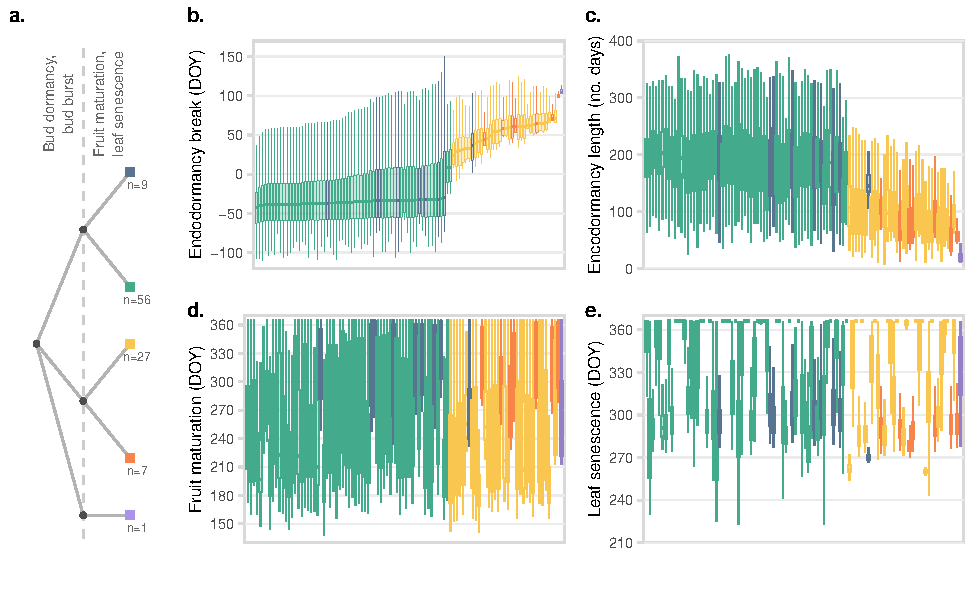
\includegraphics{fig2-1.pdf}
\caption{\textbf{(a)} Partition of the 100 \emph{full} inverse calibrations for \emph{Fagus sylvatica} after a two-step clustering. First clustering was based on the simulated leaf dormancy break and leafout dates. Second clustering was computed based on the fruit maturation and leaf senescence dates. \textbf{(b,c,d,e)} Simulated dates (day of the year, DOY) of \textbf{(b)} bud endodormancy, \textbf{(c)} bud ecodormancy, \textbf{(d)} fruit maturation and \textbf{(e)} leaf senescence. Colors correspond to the different clusters in \textbf{(a)}. Note that we do not show flowering as it occurs almost simultaneously with leaf unfolding.}
\label{fig:2}
\end{figure}

%\item These can lead to model outputs which are unrealistic \\
%$\rightarrow$ Figure: RMSE on phenological dates \\
%$\rightarrow$ Figure: XY plot flowering/maturation \\
%$\rightarrow$ But some are not so bad...

\begin{figure}[htpb]
\hspace*{-1cm}
\centering
\begin{subcaptiongroup}
\phantomcaption\label{fig:3A} 
\phantomcaption\label{fig:3B}
\phantomcaption\label{fig:3C}
\phantomcaption\label{fig:3D}
\phantomcaption\label{fig:3E}
\end{subcaptiongroup}
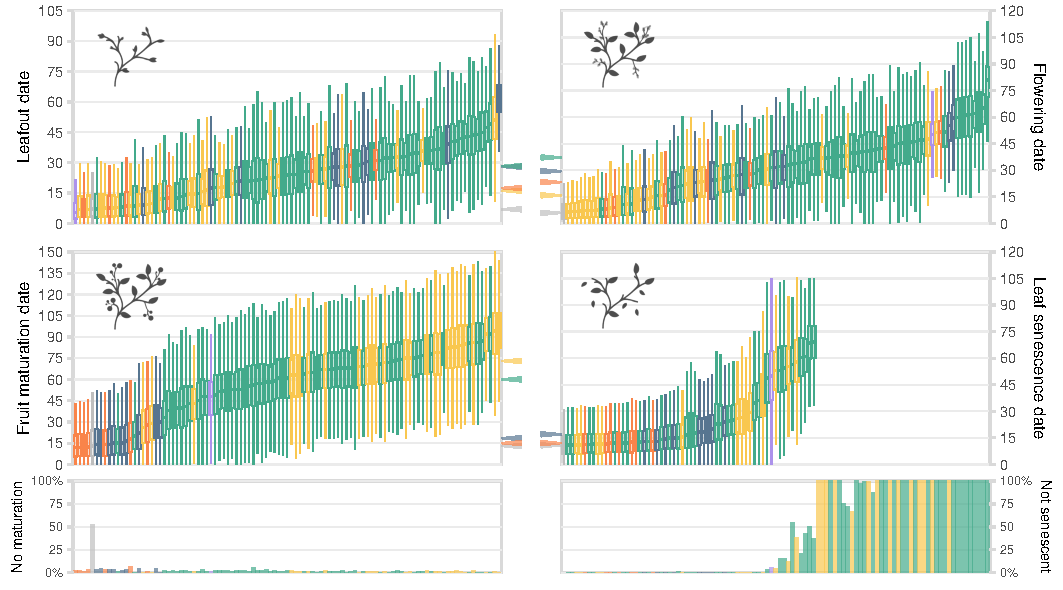
\includegraphics{fig4-1.pdf}
\caption{Root-mean-square error (RMSE) between phenological dates that were observed for \emph{Fagus sylvatica} between 1970 and 2000 and those that were predicted by the 100 \emph{full} inverse calibrations, for \textbf{(a)} leaf unfolding, \textbf{(b)} flowering, \textbf{(c)} fruit maturation and \textbf{(d)} leaf senescence. For fruit maturation and leaf senescence, the lower panels show the percentage of cases (year x site) for which the parameter sets predict that the event does not occur (i.e. no maturation or no leaf senescence). Colors are based on the clustering shown in Fig. 2, grey corresponds to the expert parameter set. Arrows in the middle indicate the median RMSE for each group.}
\label{fig:3}
\end{figure}

\subsection{Partial calibrations on selected parameters}

The previous results showed significant differences between the calibrations in terms of simulated processes and of agreements with the available observations. However, some of the calibrations simulated processes that were relatively consistent with observations, and this was confirmed in the following when attempting to inversely calibrate the processes causing false absence errors with the expert version of the model. Most partial calibrations resulted in an AUC higher than 0.8 (\Cref{fig:4}), and in the best-case scenario an increase of more than 0.4 for spruce \emph{(Picea abies}), where we transitioned from a model worst than random to one with a good discriminatory ability.

The lack of data, particularly for fruit maturation, prevented us from checking the realism of partial calibrations for all species. We were able to evaluate the inverse calibrations of the fruit maturation date submodel for beech (\emph{\emph{Fagus sylvatica} }) and pedunculate oak (\emph{Quercus robur} ) (\Cref{fig:5A}), of the flowering date submodels for birch (\emph{\emph{Betula pendula} }) and spruce  (\emph{\emph{Picea abies} }) (\Cref{fig:5B}), and the frost hardiness submodel for fir (\emph{\emph{Abies alba} }), beech and birch (\Cref{fig:5C}). For beech, most calibrated parameter sets converged towards a median error of the fruit maturation date ranging from 11 to 16 days (except one with a median error of 24 days), close to the expert version error of 13 days (\Cref{fig:5A}). Similarly to the full calibrations, they also corrected the non-fruit maturation issue of the expert version. For pedunculate oak , half of the calibrations led to errors in the fruit maturation date similar to the expert version, around 16 days, and only 9.67 days [4.33 - 17] for the best parameter set (\Cref{fig:5A}). Regarding the flowering date of birch, 2 out of 10 partial calibrations resulted in a lower median error (5.91 days [2.55 - 11.6] and 5.91 days [2.72 - 11.4]) than the expert parameter set (8.87 days [4.21 - 14.9]). However, some had a much higher median error, up to 50.2 days (\Cref{fig:5B}). For spruce, the best calibration in terms of RMSE simulated no flowering in 37.3\% of the cases. Apart from this one, the other 9 calibrations had a higher median error (between 18.3 days [10.3 - 27.9] and 29.7 days [20.0 - 41.7]) than the expert version of the model (11.5 [5.68 - 18.9]). Finally, the frost resistance submodel parameter estimates were very close to the expert version value based on the literature in only one third of the cases (\Cref{fig:5C}).

%\item Partial calibration can be a way to improve model performance \\
%$\rightarrow$ Figure: different tests of partial calibration on \emph{Fagus sylvatica} \\
%$\rightarrow$ and other species

%\begin{figure}[htpb]
%\centering
%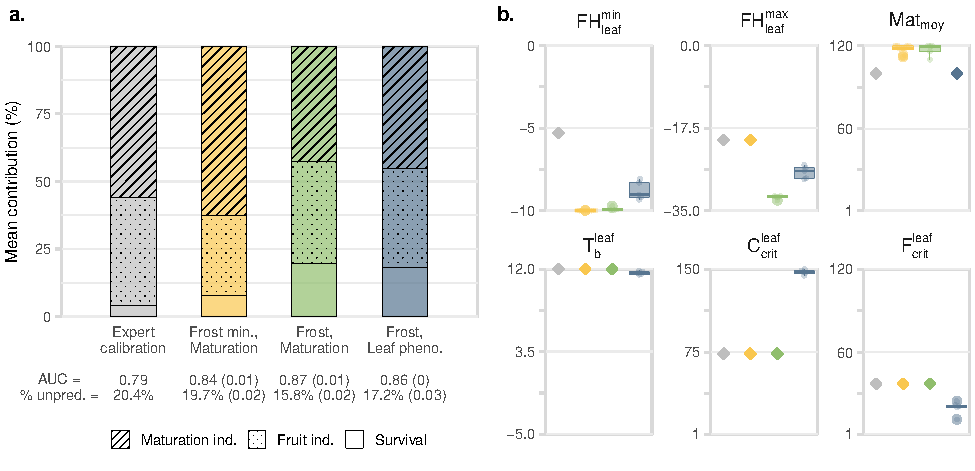
\includegraphics{fig5-1.pdf}
%\caption{Partial calibrations on \emph{Fagus sylvatica.}}
%\label{fig:partcalfagus}
%\end{figure}

\begin{figure}[htpb]
\hspace*{-0.5cm}
\centering
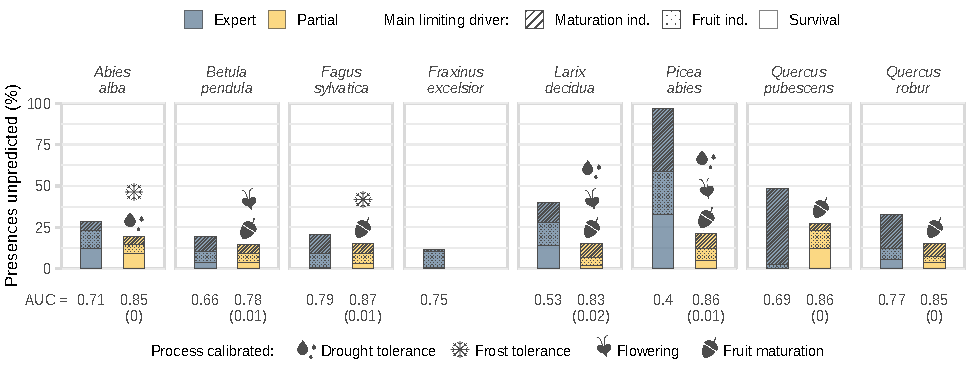
\includegraphics{fig6-1 - icons.pdf}
\caption{Results of the \emph{partial} calibrations for the eight species considered, where only some of the parameters were optimized (pictograms indicate which processes have been recalibrated using species distribution data). The y-axis shows the percentage of observed presences that are predicted as absences by the model (i.e. \emph{false absences}), and the bar patterns represent the main simulated processes explaining these errors. The bottom row shows the average AUC (a classic discrimination performance metric) and its standard deviation in parenthesis.}
\label{fig:4}
\end{figure}

%\end{itemize}

\section{Discussion}

Our results show that inverse calibration of process-explicit models (PEMs) using species distribution data does not necessarily lead to realistic parameters and simulated processes. They further demonstrate that inverse calibration can be highly useful as a model diagnostic tool, and, more importantly, to calibrate selected parts of a model where specific data and expert knowledge are lacking, albeit important cautions.

\subsection{Inverse calibration can lead to accurate species range predictions despite unrealistic parameter estimates}

% Some parameter sets outperformed the expert calibrations used for this study (especially when few data are available for the expert calibration) when predicting species distributions, but most resulted in larger errors when predicting the dates of the phenological events---up to 2 months in the worst case (\Cref{fig:3}).
Few parameter sets outperformed the expert calibrations used for this study (especially when few data are available for the expert calibration), but most resulted in larger errors when predicting the dates of the phenological events---up to 2 months in the worst case (\Cref{fig:3}).
For some other processes, inverse calibration induced even unrealistic functional traits. For example, a large portion of the calibrations considered beech as an evergreen species, or at least not senescent, in some regions (\Cref{fig:3D}).

Despite similar predictions of species distribution (\Cref{fig:1B}), we observed that simulated processes could strongly diverge between calibrated models. Some calibrated models led for example to a short endodormancy phase, followed by a longer ecodormancy phase, and \textit{vice-versa} (\Cref{fig:2A,,fig:2B}). This arises because the compensation between these two processes has little effect on the functional trait they regulate, the leaf unfolding date, and thus on the predicted distributions. The non-identifiability of parameter values obtained with inverse calibration---i.e. when different sets of parameters may result in equivalent model outputs---is a known issue \citep{He2017, Cameron2022, VanderMeersch2023}. Here we show that compensations can occur between components of a same process or between different processes. For example, errors between simulated and observed leafout dates vary greatly across calibrated models (\Cref{fig:3A}), suggesting that these errors are compensated by another process---for example, leaf frost hardiness or fruit development. 

Unexpectedly, these discrepancies in the simulated individual processes did not cause a sharp increase in the dissimilarity between the predictions of the different calibrated models over the Holocene (\Cref{fig:1C,,fig:1D,,fig:1E}), even in the very different climatic conditions of the Early Holocene (Figure S4). In other words, while inverse calibration led sometimes to very different parameter sets and thus very different "phenotypes" (early/late budburst, deciduous/evergreen...), the predictions nevertheless remained consistent across long time scales and novel climatic conditions. Therefore, the optimization algorithm manages to find consistently a similar relationship between climatic conditions and the higher-level model output (fitness), regardless of the divergent lower-level processes (frost hardiness, fruit development, etc.). The link between climate and species distribution as captured in the occurrence data thus seems to constrain the model's behavior without necessarily capturing the realistic underlying processes. In other words, the optimization algorithm appears to accommodate the model structure, making it flexible enough to fit the data well. However, this strength of the optimization algorithm is also its weakness: the model structure and the mathematical functions used to describe the processes are not sufficient to constrain the parameter estimates. Thus, contrarily to what is usually assumed \citep{Higgins2020}, here we find that PEMs are not necessarily less flexible than correlative models because of their structure. This highlights the importance of not focusing solely on some metrics of (apparent) performance, even in novel climatic conditions, but rather investigating the intermediate outputs of the model.

%\cite{Higgins2012} modified a simple theoretical model of plant growth (initially without environmental forcing) with flexible (mostly empirical?) functions to take into account monthly bioclimatic variables. The parameters of this model were then inferred using a differential evolution genetic algorithm. It has been shown to perform better than a common correlative species distribution model outside the spatial domain used for model calibration \citep{Higgins2020}. 
% The model was designed specifically for this inverse modelling experiment: it uses only monthly environmental variables, and thus has a relatively low complexity compared to the majority of other process-explicit approaches. 
%In the same spirit, \cite{VanderMeersch2023} calibrated PHENOFIT, a more complex model running at a daily step, using only species distribution data. Model was treated as a black box, and a powerfull evolutionnary algorithm (CMA-ES) was used to optimize parameter values. This "fitted" PHENOFIT achieved a high goodness-of-fit (AUC~0.9) during calibration, and was then shown to outperform several correlative models in predicting past vegetation dynamics over the Holocene, in very dissimilar climatic conditions \citep{paperrobustnesspubliéunjourinchallah}. 
%In particular, PHENOFIT was not specifically designed for inverse calibration. The classical way of using the model is to run simulations with an "expert" set of parameter values (determined mainly from experiments and measurements), and most processes simulated within the model can be confronted with field data. 
% From Higgins 2020: "Implicit in this discussion is that the parameter estimates are constrained by the model's structure. That is, how an environmental factor influences the projected species distribution is constrained by the model's assumptions. [...] This makes the model less flexible than correlative models because the model defines a priori which environmental factors influence which physiological processes, and the functional form of this influence"

Finally, and similarly to correlative models \citep{BarbetMassin2010, Duputie2014},  PEMs are affected by the bias in the occurrence data used for the calibration. For example, all simulations predict a low fitness of \emph{Fagus sylvatica} in south-western France contrary to the expert model predictions (\Cref{fig:1B}), whereas its absence is potentially more attributable to the legacy of forest management (vast maritime pine plantations) than to truly limiting climatic conditions as the presence of some old relict beech forests in the region suggests \citep{Lafontaine2014}.

\begin{figure}[h]
\hspace*{-1cm}
\centering
\begin{subcaptiongroup}
\phantomcaption\label{fig:5A} 
\phantomcaption\label{fig:5B}
\phantomcaption\label{fig:5C}
\end{subcaptiongroup}
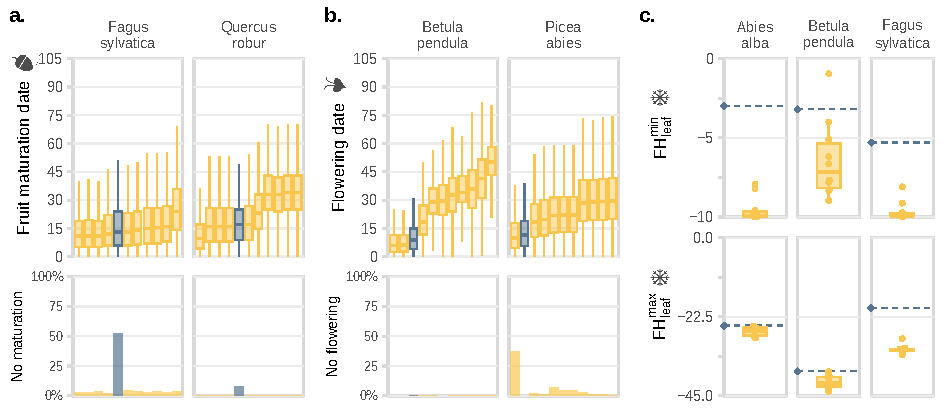
\includegraphics{fig7-1 - icons.pdf}
\caption{Root-mean-square error (RMSE) between phenological dates that were observed for the different species between 1970 and 2000 in Europe and those that were predicted by the partial calibrations (yellow) and the expert calibration (blue), for \textbf{(a)} fruit maturation and \textbf{(b)} flowering. \textbf{(c)} Distribution of the frost hardiness parameter estimates after partial calibration. The blue dotted line shows the value in the expert version of the model.}
\label{fig:5}
\end{figure}

%Brouillon, les points à évoquer:  Data bias: Landes, Pau valley \\
% $\rightarrow$ Calibrations manage to remove Fagus from there, to fit the data, even though it could be there? \\
%- les paramètres/processus sont pas très réalistes, il peut y a voir des compensatiosn très importantes... 
%- on ne peut pas croire aveuglément la calibration
% - voire même création de nouvelles espèces! Need to be careful 

\subsection{Inverse calibration can help identifying model limitations and opportunities for improvement}

Our results reveal both the power and the shortcomings of inverse calibration in ecological modeling, and call for a careful use of the method when one aims at providing projections in very different conditions from the calibration conditions. They further suggest that inverse calibration can be an effective diagnostic tool to improve PEMs, both in terms of model hypotheses and parametrization. Using species occurrence data to calibrate such models might be fruitful, if a detailed evaluation of the realism of the parameter estimates and the values of the functional traits (phenotypes) they produce is carried out.

Inverse calibration can help identify processes that are not accounted for, or incompletely accounted for in the model, even though they may be important in the context of the study.  Reversely, inverse calibration can help identify processes taken into account in the model which have little impacts on the targeted outputs. For example, the discrepancies between leaf senescence date predictions across the different calibrations (\Cref{fig:2D,,fig:3D}) highlight that, in the model, leaf senescence date is more weakly constrained by the calibration data compared to other traits because it has more limited impact on fitness. More precisely, the senescence date affects fitness if it occurs before the end of fruit development but late senescence date does not affect fitness because there is no nutrient remobilization in the model that would confer an advantage in loosing leaves before the first frost event. In this example inverse calibrations indicate that it might be opportune to refine the model by adding nutrient remobilization.

Using inverse calibration with species occurrence data can further improve PEMs in several ways. First, it can help improving the modeling of processes that have a significant impact on the model outputs but for which we have limited measurements and observations. For example, for forest tree species, observations of fruit maturation are often sparse and limited to some areas. It is therefore difficult to find the correct parameter values for the fruit maturation submodel, which can cause errors (e.g. beech, \Cref{fig:3C}). Relaxing the fruit maturation submodel parameters in the expert version of the model for several species, and calibrating them using inverse calibration and species occurrence data (\Cref{fig:4}), not only increased the model goodness-of-fit---as expected---but also resulted in more accurate predictions of fruit maturation dates on average (\Cref{fig:5A}).

Second, as pointed by \cite{Harrison2021}, the estimation of PEM parameters are sometimes \emph{ad hoc} or rely on outdated data. Thus \emph{partial} inverse calibration can also be an opportunity to identify the parameters where the disagreement between the expert value and the calibrated values is systematically significant. For example, the maximum frost resistance of beech buds during winter ($FH_{min}+\Delta FH_{max}$) is -25.3°C in the expert version of the model, while inverse calibration yields an average value of -41.4°C (\Cref{fig:5C}), which is notably lower and suggests the need to reassess the expert value. Recent studies indeed indicate values closer to -32 to -37°C \citep{Delaporte2015, Kreyling2014, Lenz2016, Baffoin2021, CharraVaskou2012}.
 
However, we should keep in mind that the parameter values inferred with such \emph{partial} calibrations are conditioned by the rest of the fixed processes and by the structural errors and hypotheses of the model. For example, the minimum frost resistance of leaves at leaf unfolding, ${FH}^{min}$, converged towards an unrealistically low value of -10°C for both beech and fir (the lower bound constraining the optimization of this parameter, (\Cref{fig:5C}). The parameters of the leaf unfolding submodel might actually be not valid for the entire study area (e.g. existence of local adaptation of populations to climatic conditions \citep{Kreyling2014}) and the calibration algorithm compensated too early leaf unfolding date with a higher frost resistance of leaves. Local adaptation could explain some variation in parameter values between expert and inversely calibrated versions of the model but not of this magnitude. More probably, this difference points to a weakness in the model, which does not account for possible different resistance to frost between a freshly unfold leaf and a mature leaf, which may have biased the estimation of ${FH}^{min}$. Parameter estimates obtained by inverse calibration using species distributions might thus also pinpoint potential improvement of the models.
% add something about Betula pendula: unlike other species, partial calibration struggle to reach an AUC>0.75 despite 3 subprocesses calibrated + high RMSE on flowering date + scattered values of FHmin (FigX) => may indicate something problematic with Betula? some process not accounted in the model? or realized distribution really does not reflect the fundamental niche?
% Finally, using occurrence data for inverse calibration can be fruitful, but nothing can spare us from "lifting the hood" and examining the processes and species on a case-by-case basis.

%Brouillon, les points à évoquer: two limitations: current parametrisation OR current model structure and hypothesis
% a diagnostic tool?
% partial calibration

\subsection{Inverse calibration can provide a more comprehensive assessment of model uncertainties}

In many applications of PEMs, parameter uncertainties are not considered and simulations are run with a single parameter sets \citep{Niu2014, Lobell2010}. Typically, in previous studies using PHENOFIT, all parameters had a chosen fixed value, and model deterministic outputs did not account for parameter uncertainties. To avoid being overconfident with individual model projections, multiple inverse calibrations could be used to generate an ensemble of model projections (Fig1b). The spread of model outputs across the ensemble may then allow to assess the uncertainty associated with the parameter values \citep{Simmonds2024}, and to provide a more comprehensive range of projections rather than single deterministic outcomes.

However, these projections will always be contingent on model hypotheses and structure. The representation of processes in models may indeed represent a large source of uncertainty, as processes can usually be modeled with various equations determining their functional form \citep{Keenan2011}. One could test a set of alternative mathematical structure to quantify the impacts of this structural uncertainty \citep{Huber2020}. An efficient way could be to include them during the calibration procedure, i.e. by also optimizing similarly plausible process formulations rather than just the parameter values, or by using highly flexible functions where the parameter values determine the function type.

%CA MANQUQE D'UNE TOUTE PETITE CONCLUSION QUI REPREND LES TAKE HOME MESSAGES

Overall, inverse calibration using species distribution data show promise as a method to enhance specific model components in the absence of more precise data. However, process-explicit model structure and mathematical functions alone do not sufficiently constrain the calibration process. To avoid producing unrealistic parameter estimates, inverse calibration thus necessitates a careful application and a thorough evaluation to ensure realistic modeling outcomes. 

A more robust application of inverse modeling would involve integrating diverse types of data simultaneously, in a multi-objective fashion, to leverage complementary information from various sources \citep{Cameron2022}. In the near future, the increasing availability of high-resolution data---such as remote sensing and LiDAR---combined with an effective inverse-calibration framework will probably enable a better integration of large-scale data and ultimately a more accurate model parametrization. This could even pave the way for real-time continuous data integration and model recalibration, transforming ecological models into digital twins \citep{Koning2023}.

%we cannot distinguish between between "model-data difference due to parameter error, model structural error or observation error" (Cameron et al. 2022)

% \subsection{Idées au brouillon, en partie reprise ci-dessus:}

% \begin{itemize}

% \item We obtain different parameters/processes despite similar output simulations, high uncertainty in the parameter estimates resulting from ivnerse calibration
% $\rightarrow$ compensations \\
% $\rightarrow$ really different phenotypes... and new species (evergreen Fagus!)\\
% "inverse calibration procedure may lead to more accurate higher-level dynamics in such a situation without necessarily being based on an accurate model structure or identifying the correct corresponding parameter values" (Cailleret et al. 2019) \\
% we cannot distinguish between between "model-data difference due to parameter error, model structural error or observation error" (Cameron et al. 2022) and optimization algorithm "has no means to change the structure of the model" (ça serait possible? à creuser!)

% \item Data bias: Landes, Pau valley \\
% $\rightarrow$ Calibrations manage to remove Fagus from there, to fit the data, even though it could be there? \\

% \item Offering insights into model limitations, identify where it should be improve, i.e. prospects for the model?\\
% $\rightarrow$ e.g. no impact of senescence \\
% closely connected to structural model error\\
% "processes or drivers that are not accounted for by the model (exogenous uncertainties)"\\
% $\rightarrow$ We did not test model uncertainty directly though, any projections will always be contingent on model structure. Possible to try a "set of alternative formulations (ensemble simulations) to quantify the impacts of structural uncertainty" (Huber et al. 2020), but the best would be to include it during the optimization process, i.e. also optimized similarly plausible process formualtions \\
% "Any given process can usually be modeled in a variety of ways (e.g., the —in terms of how processes and states are connected to, or feed back upon, each other—and the functional form of the relationship between processes and drivers)" (Keenan et al. 2011, Oecologia), it would be possible theoretically to test for model uncertainty ? => the most difficult to identify and quantify? \\
% And beware of the fixed internal relations (could be included as variables in the optimization process ?)

% \item Estimate parameter/model uncertainty ranges  \\
% the parameter uncertainty is commonly ignored, and the simualtions are run with a single parameter sets (https://doi-org.inee.bib.cnrs.fr/10.1016/j.agrformet.2010.07.008) \\
% future uncertainty is mostly adressed through simulations based on multiple GCMs - but with one model, one parameter set? \\
% "using fixed values for all the parameters in one deterministic model does not account for uncertainty in the parameters and state variables" (Niu2014) => PHENOFIT : each input parameter has a chosen fixed value, and we get a single output of the model \\
% Thus interesting to compare direct (prior) and inverse (posterior) parameter estimates and resulting processes...\\

% \item When used carefully, partial calibration can improve model goodness-of-fit while infering realistic parameter values? \\
% Two possibilities to add more constraints with the same data: fix some parameter values/processes or narrow the ranges? \\
% Can help to get a closer integration of data, "model parameter estimation tends to be ad hoc and is frequently based on single values for ‘model’ species that are long outdated" (S. Harrisson), e.g. FHmax Fagus?\\
% Check parameter realism however: e.g. FHmin -> -10 (too low? due to no difference between young/mature leaves? => model limitations)

% \item multiple calibrations: avoiding being overconfident with individual model projections, avoiding one deterministic trajectory about the future behavior of the system: "intercomparison studies that use data-informed models would be a significant step toward rigorously assessing errors due to model process representation" (Keenan et al. 2011) \\
% $\rightarrow$ model process representation indeed represent a large source of uncertainty?\\
% $\rightarrow$ increased realism is of little value if it is accompanied by over-parameterisation and ever-increasing parameter uncertainty (Harrison et al 2021) \\

% \item perspective: calibrating process-explicit models using multiple constraints (Cameron et al. 2022), integration of various sources of knowledge \\
% example: assimilating several data streams simultaneously, reduce potential overfitting issues (Bacour et al. 2023)\\
%  $\rightarrow$ but need to look at "the imbalance before the calibration starts", "the underlying issue is not one of sample size or information content per se" but rather related to "model structural deficiencies and data systematic biases"\\
%  + How to  account for spatial variability? (local adaptation)\\
%  various spatial resolution datasets ? \\
%  "cost function for each data stream passes a χ2 test (at 90\% confidence) for acceptance/rejection (after variance normalization based on the minimum cost function obtained (e.g., Franks et al., 1999; Richardson et al., 2010). This approach is preferable to using the aggregate cost function, as it ensures that model predictions are consistent with each of the individual data streams." (Keenan et al. 2012), each data stream is given equal importance in the optimization \\
%  $\rightarrow$ conducting a synthetic experiment with data is also a way to validate the ivnerse calibration framework (Keenan et al. 2011, Oecologia)

%  \item recent emergence of new data sources offers new opportunities and raises new questions for the use of inverse modeling? \\
%  (but need to be careful when adding complexity... it may not necessarily be the objective to aim for)
    
% \end{itemize}

% Bayesian OK but : "single posterior (direct estimates as informative prior) did not qualitatively change the results compared to the uninformative inversion, as the inverse signal (likelihood) was substantially stronger than the prior (i.e., the posterior parameter estimates were strongly informed by the data)" (Cailleret et al. 2019)\\
% + bayesian method using very flat prior PDF generates results close to those estimated by a "frequentist" method (Chapter 7 - Parameter Estimation with Bayesian Methods’. In Working with Dynamic Crop Models (Second Edition)) $\rightarrow$ need to use more informative priors, such as in Heiland et al. (prior from Slovakia applied to Germany) \\
% + from Keenan et al. 2011: a confidence interval should be conditional on both data and the model, BUT if "a confidence interval is conditional on both data and the model", what do the uncertainty estimates really represent?

\end{linenumbers}
\end{doublespacing}

%%%%%%%%%%%%%%%%%%%%%%%%%%%%%%%%%%%%%%%%%%%%%%%%%%%%%%%%%%%%%%%%%%%%%
%\section{Acknowledgments}
%%%%%%%%%%%%%%%%%%%%%%%%%%%%%%%%%%%%%%%%%%%%%%%%%%%%%%%%%%%%%%%%%%%%%
%\lipsum[13] 


%%%%%%%%%%%%%%%%%%%%%%%%%%%%%%%%%%%%%%%%%%%%%%%%%%%%%%%%%%%%%%%%%%%%%
%\section{Author Contributions}
%%%%%%%%%%%%%%%%%%%%%%%%%%%%%%%%%%%%%%%%%%%%%%%%%%%%%%%%%%%%%%%%%%%%%
%Conceptualization: Methodology: Investigation: Visualization: Writing:  Editing: Funding Acquisition: Supervision: . 

%\section{Author Competing Interests}
%\lipsum[14][2]

%%%%%%%%%%%%%%%%%%%%%%%%%%%%%%%%%%%%%%%%%%%%%%%%%%%%%%%%%%%%%%%%%%%%%
\renewcommand\refname{References}
%%%%%%%%%%%%%%%%%%%%%%%%%%%%%%%%%%%%%%%%%%%%%%%%%%%%%%%%%%%%%%%%%%%%%
\begin{footnotesize}
%\renewcommand{\bibnumfmt}[1]{#1.}
\bibliographystyle{spbasic.bst} % abbrvnat or unsrt
\textnormal{\bibliography{contrast.bib}}
\end{footnotesize}
\newpage


%%%%%%%%%%%%%%%%%%%%%%%%%%%%%%%%%%%%%%%%%%%%%%%%%%%%%%%%%%%%%%%%%%%%%
% Tables
%%%%%%%%%%%%%%%%%%%%%%%%%%%%%%%%%%%%%%%%%%%%%%%%%%%%%%%%%%%%%%%%%%%%%

%\newpage
%\include{table.tex}

%%%%%%%%%%%%%%%%%%%%%%%%%%%%%%%%%%%%%%%%%%%%%%%%%%%%%%%%%%%%%%%%%%%%%
% Figures
%%%%%%%%%%%%%%%%%%%%%%%%%%%%%%%%%%%%%%%%%%%%%%%%%%%%%%%%%%%%%%%%%%%%%
%%%%%%%%%%%%%%%%%%%%%%%%%%%%%%%%%%%%%%%%%%%%%%%%%%%%%%%%%%%%%%%%%%%%%%
% Figures
%%%%%%%%%%%%%%%%%%%%%%%%%%%%%%%%%%%%%%%%%%%%%%%%%%%%%%%%%%%%%%%%%%%%%

\newpage

%%%%%%%%%%%%% Figure 1
\begin{figure}
\centering
\begin{subcaptiongroup}
\phantomcaption\label{fig:1A} % add one of these for each subpanel
\phantomcaption\label{fig:1B} % add one of these for each subpanel
\end{subcaptiongroup}
\includegraphics[width=1\textwidth]{figures/sampfig.png}
\caption{\textcolor{Highlight}{\textbf{Schematic illustrations of apparatus design.}}\\
(A)
Some text.\\
(B)
More text.\\
(C) 
Last text.
}
\label{fig:F1}

\end{figure}

%%%%%%%%%%%%%%%%%%%%%%%%%%%%%%%%%%%%%%%%%%%%%%%%%%%%%%%%%%%%%%%%%%%%%
% SUPPLEMENTAL Figures
%%%%%%%%%%%%%%%%%%%%%%%%%%%%%%%%%%%%%%%%%%%%%%%%%%%%%%%%%%%%%%%%%%%%%

\beginsupplement % <- renumbers everything and starts figure naming with "S" per local.sty
\end{document}